\documentclass[aspectration=1610]{beamer}

\usetheme{Hannover}
\usecolortheme{rose}
\definecolor{JagBlue}{HTML}{00205B}
\definecolor{JagRed}{HTML}{BF0D3E}

\usepackage{tikz,pgfplots}

%Center frame titles
\setbeamertemplate{frametitle}[default][center]

\title{Welcome to Linear Algebra}
\author{Dr. Lewis}

\date{Spring 2020}


\begin{document}

\begin{frame}
\titlepage
\end{frame}

\begin{frame}\frametitle{Team-Based Inquiry Learning}
This course uses Team-Based Inquiry Learning and Standards Based Grading.
\begin{itemize}
	\item There is a large body of research supporting the effectiveness of TBIL.
	\item There is a large body of research supporting the effectiveness of SBG.
	\item Today we will discuss how and why these pedagogies are implemented in this class.
\end{itemize}
  
\end{frame}
 
\begin{frame}\frametitle{Teams}
Everybody stand up!
  
\begin{itemize}
\item Based on your responses to the survey, I have organized you into teams.
\item I did this pseudo-randomly, ensuring a mix of majors on each team.
\end{itemize}
\end{frame}

\begin{frame}\frametitle{Team Names}
\begin{itemize}
\item Introduce yourselves to each other
\item Decide on a name for your team
\item Elect a team member to stand up and introduce each team member to the class.

\end{itemize}
\end{frame}






\begin{frame} \frametitle{What is Linear Algebra? }
Linear algebra is the study of {\bf linear maps}.
\begin{itemize}
\item In Calculus, you learn how to approximate any function by a linear function.
\item In Linear Algebra, we learn about how linear maps behave.
\item Combining the two, we can approximate how any function behaves.
\end{itemize}
\end{frame}

\begin{frame} \frametitle{What is Linear Algebra good for?}
\begin{itemize}
\item In an abstract sense, linear algebra is arguably the most used tool in higher math.
\item In computer graphics, linear algebra is used to help represent 3-dimensional objects in a two dimensional grid of pixels.
\item Differential equations are often very difficult (or impossible) to solve exactly; we use linear algebra to understand approximate solutions in a vast number of engineering applications such as fluid flows, vibrations, heat transfer, etc.
\item Google's famed Page Rank algorithm is based on linear algebra
\item Sports rankings 
\end{itemize}
\end{frame}

\begin{frame} \frametitle{Learning Outcomes }
By the end of this class, you will be able to
\begin{itemize}
\item Work collaboratively on difficult mathematics problems
\pause \item Solve systems of linear equations.
\pause \item Determine whether or not a set with given operations is a vector space or a subspace of another vector space.
\pause \item Determine properties of sets of vectors such as whether they are linearly independent, whether they span, and whether they are a basis.
\pause \item Perform fundamental operations in the algebra of matrices, including multiplying and inverting matrices.
\pause \item Use and apply algebraic properties of a linear transformation.
\pause \item Determine geometric information about a linear transformation, including computing determinants, eigenvalues, and eigenvectors.
\end{itemize}
\end{frame}





  \section{Team-Based Learning (TBL)}

  \begin{frame}\frametitle{Team-Based Learning}
  In this class we will use {\bf Team-Based Learning}.
  \begin{itemize}
    \item Research shows that TBL leads to improved student learning.
  \end{itemize}

\begin{center}
    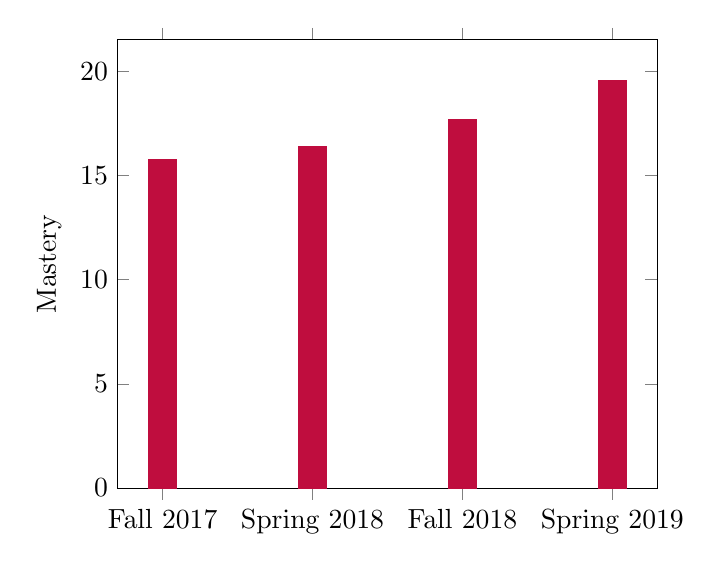
\begin{tikzpicture}
    \begin{axis}[ybar, symbolic x coords = {Fall 2017, Spring 2018, Fall 2018, Spring 2019},ymin=0, xtick=data, ylabel={Mastery}]
    \addplot[color=JagRed,fill=JagRed] coordinates { (Fall 2017, 15.77) (Spring 2018, 16.4) (Fall 2018, 17.7) (Spring 2019, 19.56)};
    \end{axis}
    \end{tikzpicture}
\end{center}  

  \end{frame}
  

  
  \begin{frame}\frametitle{TBL Improves Course Grades}
  
  \begin{center}
  \includegraphics[scale=0.5]{grades.png}
  \end{center}
  \end{frame}
  
  \begin{frame}\frametitle{Overview of TBL}
  \begin{itemize}
  \item The course is divided into 5 ``modules''.
  \item The first day of each module is the Readiness Assurance Process.
  \item Remaining days are spent working on activities in your teams.
  \end{itemize}
  \end{frame}

  \begin{frame}\frametitle{Readiness Assurance Process}
  \begin{itemize}
  \item In USAOnline, you will find a list of the skills you should have {\bf before each module starts}, along with resources to help you prepare.
  \begin{itemize}
  \item Sometimes these skills are from previous courses.
  \item Sometimes these skills are standards from earlier in this course.
    \item Sometimes (but rarely) these are new skills you will learn by watching the videos and answering embedded questions.
  \end{itemize}
  \pause \item On the first day of the module, the Readiness Assurance Tests will ensure you have these skills.
  \begin{itemize}
  \item First, you will individually take the RAT
  \item After everyone is done, you will take the RAT again collaboratively as a team.
  \end{itemize}
  \item {\bf The first Readiness Assurance day is Wednesday!}
  \end{itemize}
  \end{frame}
  
  
\begin{frame}\frametitle{Class Activities}
Most days we will spend our time working in teams through a series of activities on the whiteboards.
\begin{itemize}
\item These activities are designed to help you \textbf{explore} the material.
\item Often, you will not immediately know how to complete them.  You will have all the tools you will need, but will have to apply them in a new way.
\item Sometimes, it will be hard.  That's okay!
\item Research shows these kind of activities lead to deeper learning.
\end{itemize}

\end{frame}
  

\begin{frame}\frametitle{Team and Class Norms}

In your teams, come up with a list of norms you would like your team (and the class to follow)
\vfill
What things do you want your teammates to do this semester, and what should they expect of you?
\vfill
\end{frame}

\begin{frame}\frametitle{Peer evaluations}


\begin{itemize}
\item At several points in the semester, you will evaluate and offer anonymous feedback to your teammates.
\item I will remind you of the class norms we just agreed upon and ask you to reflect how your teammates are upholding the norms.
\end{itemize}
\end{frame}

\section{Standards Based Grading (SBG)}
\begin{frame}\frametitle{What does a grade represent?}

In your teams, make a list of all the things a grade in a course represents.
\vfill

\pause
What should a grade represent?
\vfill
\end{frame}



\begin{frame}\frametitle{Standards Based Grading (SBG)}
Your main job in this course is to \textbf{master the covered material}
and \textbf{demonstrate that mastery to me}.

\vspace{0.2in}
\pause

You will be given several opportunities to demonstrate mastery throughout
the semester, and if
at first you don't succeed, you can try again without any penalty.
\end{frame}

\begin{frame}\frametitle{SBG is different!}
SBG has many advantages
\begin{itemize}
\item You can learn and demonstrate mastery at \textbf{your} pace, not the instructor's.
\item No high stakes exams -- you can always reassess at a later date.
\item You can demonstrate mastery in multiple ways.
\end{itemize}
\vfill
But it's different!
\begin{itemize}
\item Some students take some time to adjust.  Unlike many courses you have taken before, \textbf{you will not succeed by only accumulating partial understanding.}
\item The best advice former students give is to not delay mastering standards.
\end{itemize}
\end{frame}




\begin{frame}\frametitle{SBG}
The course material is broken down into 24 learning \textbf{standards}.
\begin{itemize}
\item Each attempted exercise will be simply marked according to whether or not
      your solution demonstrates mastery of the relevant standards.
\item Each solution that demonstrates complete mastery counts as a
      \textbf{checkmark} for that standard.
\item Up to two checkmarks may be earned for each standard. Your grade depends
      on the total number of checkmarks you earn this semester (up to 48).
\item Standards will be assessed several times, and there's no penalty for
      incorrect solutions. So, if you don't succeed the first time,
      keep practicing and try again!
\end{itemize}
\end{frame}

\begin{frame}\frametitle{Assessment Opportunities}
Checkmarks may be earned as follows.
\begin{itemize}
\item {\bf Quizzes}: Most weeks, one day at the end of class we will have a quiz. 
\item {\bf Exams}: Periodically we will have longer assessments (usually on Friday).
\item {\bf Final Exam}: Your final opportunity to demonstrate mastery,
      cumulative over the entire course.
\item {\bf Office Hours Reassessments}: A limited number of opportunities
      will be provided to earn checkmarks outside of class.
\end{itemize}

\pause

\vspace{0.2in}

The assessment method (quiz/exam/etc.) you used to earn a checkmark
isn't important: \textbf{I only care that you
learn the material and demonstrate that mastery to me before the end of the
semester!}
\end{frame}

\begin{frame}\frametitle{A tale of two students}
These two students took very different paths, but both earned the same grade.
\begin{center}
\includegraphics[scale=0.7]{student-comparison.png}
\end{center}
\end{frame}



\begin{frame}\frametitle{Interpreting Feedback}
On each assessment, for each standard you will receive one of the following marks.
\begin{itemize}
\item {\bf M} means you demonstrated \textbf{Mastery} of that standard.
      Great job!  Check off another box on your progress sheet.
\item {\bf *} means you have a minor mistake, but if you can come by my office hours and explain it,
      this mark will be changed to {\bf M}.
\item {\bf W} means you have demonstrated understanding, but not written a complete solution.  Often, notation is poor or ambiguous.  You can provide a {\bf Written} re-working of the same problem (fixing any errors) to earn an {\bf M}.
\item {\bf R} means you made a good faith effort and demonstrated
      partial understanding, but not complete mastery. You are eligible to
      \textbf{Reattempt} the standard outside of class.
\item {\bf N} means there was \textbf{No Significant Evidence} of understanding.
\end{itemize}

\vspace{0.2in}

Marks other than M do not improve your course letter grade, but
they don't hurt you either.
\end{frame}




\begin{frame}\frametitle{Course Grades}

\begin{center}
\begin{tabular}{ll} \hline
A & Earn 45 mastery checkmarks.\\ \hline
B & Earn 40 mastery checkmarks. \\ \hline
C & Earn 35 mastery checkmarks.\\ \hline
D & Earn 30 mastery checkmarks. \\ \hline
\end{tabular}
\end{center}

\end{frame}


\begin{frame}\frametitle{Other Assessments}
In addition to mastering content, I will ask you to do some other things because experience shows these help students learn.
\begin{itemize}
\item Class Attendance
\item Individual \& Team Readiness Assurance Tests
\item Peer Evaluations
\item Self Assessments
\item Homework
\end{itemize}
\end{frame}






\begin{frame}\frametitle{Office Hours (Student Hours)}
Office Hours are meant to be for the following things (among others):
\begin{enumerate}
\item Questions
\item Conversations
\item Reassessments
\end{enumerate}

\vspace{0.2in}

{\bf Office Hours (drop-in) are MWF 8:15-9:00 and 10-11}.  If you can't make these times, send me an email for an appointment.

\vspace{0.1in}
My office is room 439 (upstairs).

\end{frame}



\begin{frame}\frametitle{Homework}
Homework is practice.  A list of homework exercises, organized by standard, is available in Campuswire.
\begin{itemize}
\item I will not collect or grade homework.
\item You will need to show me your homework in order to reassess in my office hours
\item If you need help or feedback, come to my office hours or post in the class discussion site.
\end{itemize}
\end{frame}

\begin{frame}\frametitle{Campuswire}
We will be using an online discussion site called Campuswire this semester.
\begin{itemize}
\item After you work an activity in class, one team member should take a picture of your whiteboard, and upload it to Coursewire later that day.
\item If your whiteboard solution for an activity is incomplete or incorrect, your team should add a correct solution.
\item There is also space to ask questions about the content or the class; you are encouraged to answer your classmates' questions!
\end{itemize}

\end{frame}

\begin{frame}\frametitle{Questions}

\begin{itemize}
\item Will this be a class that makes me want to learn more? 
\item Can we please pick our own groups?
\end{itemize}
\end{frame}


\begin{frame}\frametitle{Reminder}
The first Readiness Assurance Day is Wednesday!!!
\end{frame}



\end{document}
